\documentclass[a4paper, 12pt]{book}
\usepackage[margin=2.5cm]{geometry}
\usepackage[italian]{babel}
%\usepackage{wrapfig}
\usepackage{graphicx}   % per inserire immagini
\usepackage{caption}    % per le didascalie
\usepackage{subcaption} % per sottodidascalie
\usepackage[normalem]{ulem}   % per sottolineare, barrare o marcare
\usepackage{hyperref}
\usepackage{float}
\usepackage{amsmath}
\setlength{\parindent}{0pt}
\usepackage{parskip}
\usepackage{soul}
\usepackage{xcolor}
\sethlcolor{yellow}
\usepackage{array}\usepackage[most]{tcolorbox}
\usepackage{booktabs}
\usepackage{tikz}
\usetikzlibrary{positioning}
\usepackage{longtable}
\usepackage{array}
\usepackage{fancyhdr}
\setlength{\headheight}{15pt}
\pagestyle{fancy}
\fancyhf{} % pulisce header e footer
\fancyhead[R]{\thepage} % numero pagina a destra nell'header
\renewcommand{\headrulewidth}{0pt} % (opzionale) elimina la riga orizzontale sotto l'header
\fancypagestyle{plain}{%
  \fancyhf{} % pulisce header e footer
  \fancyhead[R]{\thepage} % numero sempre in alto a destra
  \renewcommand{\headrulewidth}{0pt} % opzionale: niente linea
}
\setcounter{tocdepth}{3}

\title{\textbf{Basi di dati - primo semestre}\\uniVR - Dipartimento di Informatica}
\author{Mattia Nicolis \and Matteo Drago}
\date{A.A. 2025-26}

\begin{document}

    \maketitle

    \tableofcontents
    \markboth{}{}

    %-------MODULO DI TEORIA------------------------------------
    %-------Prof: Alberto Belussi-------------------------------
    %-------Lez: Martedì (10:30-12:30) [Aula A - Cav.1]----------
    %-------Lez: Venerdì (11:30-13:30) [Aula A - Cav.1]----------

    \chapter*{Introduzione}
    \addcontentsline{toc}{chapter}{Introduzione}

    \section*{Storia delle DBMS}
    \addcontentsline{toc}{section}{Storia delle DBMS}


    La nascita dei sistemi per la gestione di basi di dati ha visto due momenti principali:
    \begin{description}   % Ambiente description, [parola] in grassetto 
      \item \textbf{anni '60}: sviluppo di applicazioni negli \textbf{ambienti di ricerca scientifica}
      \item \textbf{anni '70}: sviluppo di applicazioni informatiche in \textbf{ambito gestionale}
    \end{description}

    Si trattava di semplici dispositivi in cui gli \uline{algoritmi} di elaborazione \uline{erano semplici} e \uline{grandi quantità di dati} erano \uline{\textbf{condivisi}} da più applicazioni.
    
    Queste caratteristiche erano specifiche per l'ambiente in cui erano state introdotte ovvero il \textbf{sistema informativo}.


  %------------BLOCCO DEFINIZIONE--------------------%

    \vspace{15pt}

    \begin{tcolorbox}[
      colback=cyan!5!white,
      colframe=blue!50!black,
      title=\textbf{Definizione - Sistema informativo},
      coltitle=white,
      fonttitle=\bfseries,
      arc=3mm,
      boxrule=0.5pt,
      enhanced,
      breakable
    ]
    L'insieme delle attività umane e dei dispositivi di memorizzazione ed elaborazione che organizza e gestisce l'informazione di interesse per una organizzazione di dimensioni qualsiasi.\\
    
    \vspace{0.5mm}
    
    \textbf{N.B: non per forza è contenuta tecnologia informatica}
    \end{tcolorbox}

    \vspace{15pt}

  %--------------------------------------------------%


    Il sistema informativo è costituito da \textit{dati} e \textit{informazioni}:
    \begin{itemize}
      \item \textbf{dato}: elemento di conoscenza di base costituito da simboli che devono essere elaborati
      \item \textbf{informazione}: interpretazione dei dati che permette di ottenere conoscenza più o meno esatta di fatti e situazioni
    \end{itemize}
    
    Lo studio del sistema informativo avviene attraverso i \textbf{diagrammi di flusso}, questi permettono di svolgere diverse operazioni tra cui: 
    \begin{itemize}
      \item definizione archivi dati e delle sorgenti di dati
      \item definizione degli utenti
      \item definizione di procedure e processi
      \item definizione dei flussi dati
    \end{itemize}


    \clearpage
    \textbf{\large Come si è arrivati allo sviluppo dei DBMS?}
 
    Negli anni '70, i programmi comunicavano direttamente con i dati contenuti nel file system. 
    
    Era un'operazione scomoda in quanto l’accesso ai dati su file era scarso (\textbf{struttura ad accesso sequenziale}), c'era ridondanza nei dati (\textbf{duplicazioni dello stesso dato su più file}), inconsistenza dovuta ad aggiornamenti parziali e progettazione dei dati replicata per ogni programma.

    Negli anni '80, la soluzione che venne proposta fu quella di inserire un \textbf{DBMS} (Data Base Management System) tra il \textbf{file system} e le \textbf{applicazioni}.

    \begin{figure}[h]
      \centering

      \begin{subfigure}[b]{0.45\textwidth}
        \centering
        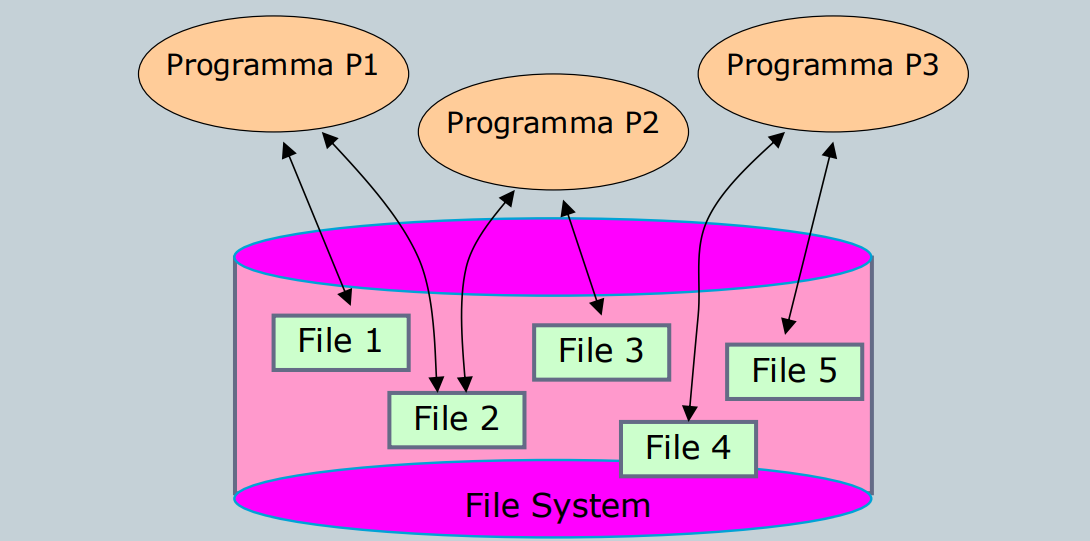
\includegraphics[width=\textwidth, height=3.8cm]{images/fileSystem.png}
        \caption{Solo file system}
      \end{subfigure}
      \hfill
      \begin{subfigure}[b]{0.45\textwidth}
        \centering
        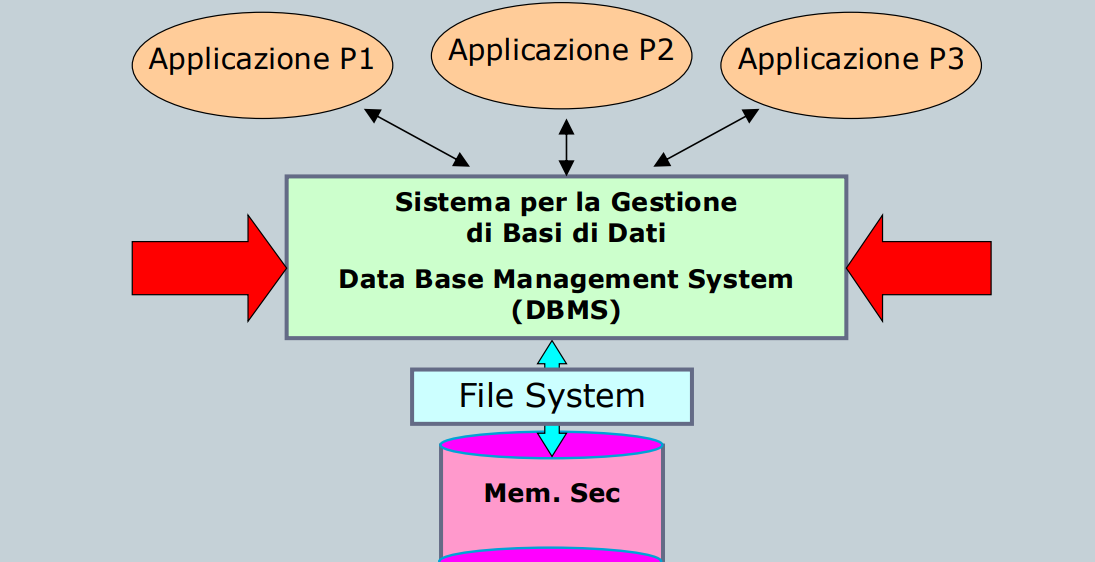
\includegraphics[width=\textwidth, height=3.8cm]{images/DBMS.png}
        \caption{File system + base di dati}
     \end{subfigure}

    \caption{Prima e dopo l'innovazione}
    \end{figure}



  %------------BLOCCO DEFINIZIONE--------------------%

    \vspace{15pt}

    \begin{tcolorbox}[
      colback=cyan!5!white,
      colframe=blue!50!black,
      title=\textbf{Definizione - Base di dati},
      coltitle=white,
      fonttitle=\bfseries,
      arc=3mm,
      boxrule=0.5pt,
      enhanced,
      breakable
    ]
    Una collezione di dati utilizzati per rappresentare con tecnologia informatica le informazioni di interesse per un sistema informativo.
    \end{tcolorbox}

    \vspace{15pt}

  %%%------------CHIUDE DEFINIZIONE-------------------%%% 

  %------------BLOCCO DEFINIZIONE--------------------%

    \vspace{15pt}

    \begin{tcolorbox}[
      colback=cyan!5!white,
      colframe=blue!50!black,
      title=\textbf{Definizione - DBMS},
      coltitle=white,
      fonttitle=\bfseries,
      arc=3mm,
      boxrule=0.5pt,
      enhanced,
      breakable
    ]
    Sistema che gestisce su memoria secondaria collezioni di dati \textbf{grandi} , \textbf{condivise} e \textbf{persistenti}, assicurandone l'\textbf{affidabilità} la \textbf{privatezza} e l'\textbf{accesso efficiente}.
    \end{tcolorbox}

    \vspace{15pt}

  %%%------------CHIUDE DEFINIZIONE-------------------%%%  


    Questo nuovo approccio ha portato numerosi vantaggi:
    \begin{itemize}
      \item \textbf{maggiore astrazione} e più potenza espressiva per descrivere le proprietà del dato.
      \hl{All'interno del \textbf{DMBS} i dati vengono interpretati come oggetti ovvero istanze di classi o righe di tabelle}.
      
      Prima erano interpretati come blocchi o pagine di memoria secondaria (sequenze di byte)

      \item operazioni di accesso ai dati più complesse basate su un linguaggio di interrogazione (SELECT FROM WHERE) anzichè attraverso operazioni di READ/WRITE
      \item migliorata l'interazione uomo-informazione: 
      \begin{itemize}
        \item linguaggio per la definizione dei dati (Data Definition Language - DDL)
        \item linguaggio per l’interrogazione e aggiornamento dei dati (Data Manipulation Language – DML): 
        \begin{itemize}
          \item linguaggio di interrogazione: estrae informazioni da una base di dati (esempio: SQL, algebra relazionale)
          \item linguaggio di manipolazione: popola la base di dati, modifica il suo contenuto con aggiunte, cancellazioni e variazioni sui dati (es. SQL)
        \end{itemize}
      \end{itemize}
    \end{itemize}

    


   %------------BLOCCO DEFINIZIONE--------------------%

    \vspace{15pt}

    \begin{tcolorbox}[
      colback=cyan!5!white,
      colframe=blue!50!black,
      title=\textbf{Definizione - DBMS: modello dei dati},
      coltitle=white,
      fonttitle=\bfseries,
      arc=3mm,
      boxrule=0.5pt,
      enhanced,
      breakable
    ]
    È l’insieme dei costrutti forniti dal DBMS per descrivere la struttura e le proprietà dell’informazione contenuta in una base di dati.
    
    \vspace{1mm}
    
    I costrutti permettono di definire le strutture dati che conterrano le informazioni e specificare le proprietà che dovranno soddisfare le istanze.

    \end{tcolorbox}

    \vspace{15pt}

  %%%------------CHIUDE DEFINIZIONE-------------------%%%  


     Nel passato esistevano modelli come quello reticolare o quello gerarchico.

     Attualmente si parla di modello relazionale, ad oggetti, object-relational (SQL99 o SQL3), basato sui documenti(JSON) o NoSQL.


%------------BLOCCO DEFINIZIONE--------------------%

    \vspace{15pt}

    \begin{tcolorbox}[
      colback=cyan!5!white,
      colframe=blue!50!black,
      title=\textbf{Definizione - Schema di una base di dati},
      coltitle=white,
      fonttitle=\bfseries,
      arc=3mm,
      boxrule=0.5pt,
      enhanced,
      breakable
    ]
    È la descrizione della struttura e delle proprietà di una specifica base di dati fatta utilizzando i costrutti del modello dei dati (lo schema di una base di dati è invariante nel tempo).

    \end{tcolorbox}

    \vspace{15pt}

  %%%------------CHIUDE DEFINIZIONE-------------------%%%  

  %------------BLOCCO DEFINIZIONE--------------------%

    \vspace{15pt}

    \begin{tcolorbox}[
      colback=cyan!5!white,
      colframe=blue!50!black,
      title=\textbf{Definizione - Istanza di una base di dati},
      coltitle=white,
      fonttitle=\bfseries,
      arc=3mm,
      boxrule=0.5pt,
      enhanced,
      breakable
    ]
    È costituita dai valori effettivi che in un certo istante popolano le strutture dati della base di dati (l’istanza di una base di dati varia nel tempo).

    \end{tcolorbox}

    \vspace{15pt}

  %%%------------CHIUDE DEFINIZIONE-------------------%%%  


    \begin{figure}[h]
        \centering
        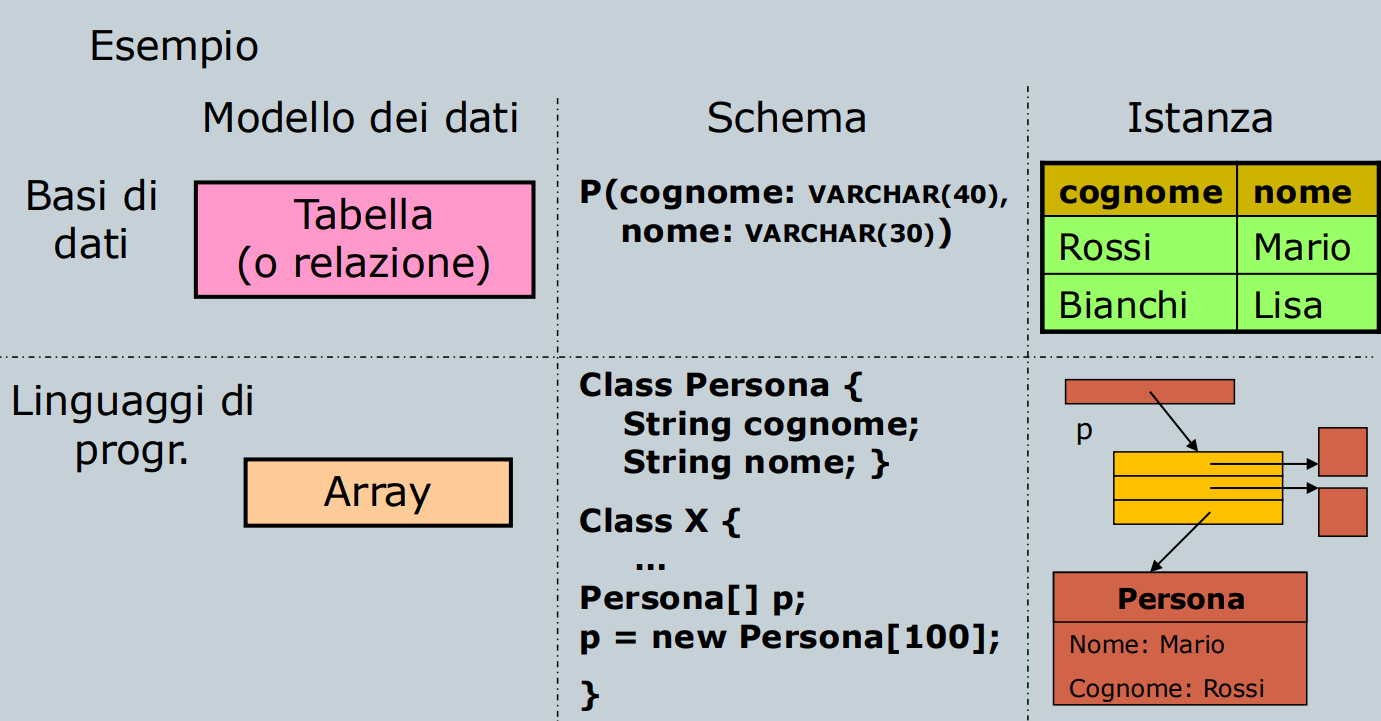
\includegraphics[width=0.8\textwidth]{images/modelloSchemaIstanza.png}
        \caption{Distinzione tra modello, schema e istanza}
    \end{figure}



    \section*{Architettura di un DBMS}
    \addcontentsline{toc}{section}{Architettura di un DBMS}

    \begin{itemize}
      \item \textbf{schema logico}: è la rappresentazione della struttura e delle proprietà della base di dati definita attraverso i costrutti del modello dei dati del DBMS
      \item \textbf{schema interno}: è la rappresentazione della base di dati per mezzo delle strutture fisiche di memorizzazione (file dati, file indice, ecc…)
      \item \textbf{schema esterno}: descrive una porzione dello schema logico di interesse per uno specifico utente o applicazione (attraverso viste sullo schema logico)
    \end{itemize}
  
    
    La caratteristica fondamentale di queste strutture è l'\textbf{indipendenza}.
    \begin{description}
      \item \textbf{indipendenza fisica}: lo \uline{schema logico} della base di dati \uline{è completamente indipendente dallo schema interno}, ne consegue che le variazioni delle strutture fisiche non impattano sullo schema logico e quindi sulle applicazioni.
      \item \textbf{indipendenza logica}: gli \uline{schemi esterni} della base di dati \uline{sono indipendendi dallo schema logico}, ne consegue che le variazioni dello shcema logico (purchè non vengano rimossi dati) non impattano sugli schemi esterni e quindi sulle applicazioni (eventualmente è necessario solo ridefinire l'espressione di derivazione).
    \end{description}
     

    \chapter*{Progettazione di una base di dati}
    \addcontentsline{toc}{chapter}{Progettazione di una base di dati}
    La progettazione di una base di dati costituisce solo una delle componenti del processo di sviluppo di un sistema informativo e va, quindi, inquadrata in un contesto più ampio: il \textbf{ciclo di vita} dei sistemi infoormativi.

    Il \textit{ciclo di vita} di un sistema informativo comprende:
    \begin{enumerate}
      \item \textbf{studio della fattibilità}: \hl{definisce (nel modo più preciso possibile) i \textit{costi} delle varie alternative} possibili e \hl{stabilisce le \textit{priorità} di realizzazione} delle varie componenti del sistema
      \item \textbf{raccolta e analisi dei requesiti}: individua e studia le proprietà e le funzionalità del sistema, producendo una descrizioe completa, ma informale, dei dati coinvolti e delle operazione su di essi.
      \item \textbf{progettazione}: si divide in
      \begin{itemize}
        \item \textit{progettazione dei dati}: descrive la struttura e l'organizzazione dei dati
        \item \textit{progettazione delle apllicazioni}: descrive in modo formale le caratteristiche dei programmi applicativi
      \end{itemize}

      Le due attività sono complememtari e possono procedere in parallelo o in cascata.

      \item \textbf{implementazione}: realizza il sistema informativo secondo la struttura e le caratteristich definite nella fase di progettazione.
      
      Viene costruita e popolata la base di dati e viene prodotto il codice dei programmi.

      \item \textbf{validazione e collaudo}: verifica il corretto funzionamento e la qualità del sistema informativo.
      
      La sperimentazione deve prevedere, per quanto possibile, tutte le confizioni operative.

      \item \textbf{funzionamento}: entra in funzione il sistema informativo ed esegue i compiti per i quali era stato originariamente progettato.
      
      Se non si verificano malfunionamenti o revisioni delle funzionalità del sistema, questa attività richiede solo operazioni di gestione e manutenzione.
    \end{enumerate}

    \begin{figure}[H]
      \centering
      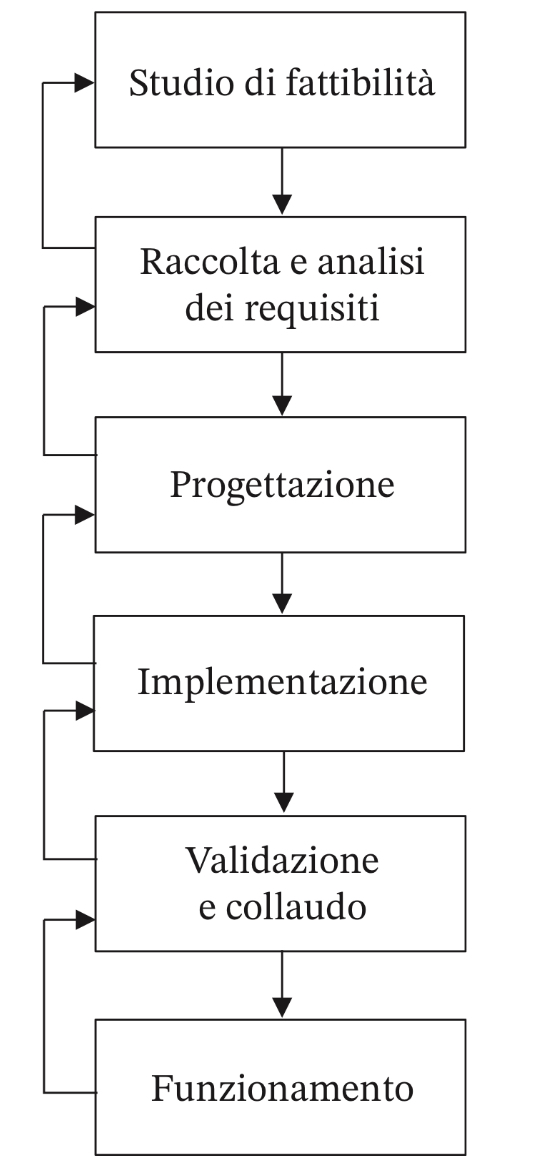
\includegraphics[width=0.2\textwidth, keepaspectratio]{images/cicloVita.jpeg}
      \caption{ciclo di vita}
    \end{figure}

    \section*{Metodologie di progettazione dei dati}
    \addcontentsline{toc}{section}{Metodologie di progettazione dei dati}
    Una \textbf{metologia di progettazione} è costituita da:
    \begin{itemize}
      \item \textbf{decomposizone} dell'intera attività di proegetto in passi sucessivi indipendeneti tra loro
      \item \textbf{insieme di strategie} da seguire nei vari passi e alcuni \textit{criteri} per la scelta in caso di alternative
      \item \textbf{modelli di riferimento} per descrivere i dati di ingresso e uscita delle varie fasi
    \end{itemize}

    Le \textit{proprietà} che una buona metologia deve avere sono:
    \begin{itemize}
      \item \textbf{generale} rispetto alle applicazioni e ai sistemi in gioco (essere inipendendete dal problema studiato e dagli strumenti utilizzati)
      \item \textbf{prodotto di qualità} in termini di \textit{correttezza}, \textit{completezza} ed \textit{efficienza} delle risorse impiegate
      \item \textbf{facile da usare} nelle strategie e neo modelli di riferimento
    \end{itemize}

    Nell'ambito delle basi di dati, si è consolidata negli anni una metodologia di proegetto che ha dato prova di soddisfare pienamente le proprietà descritte.

    Tale metodologia è articolata in tre fasi principali da effettuare a cascata:
    \begin{itemize}
      \item \textbf{progettazione concettuale}: rappresenta le specifiche informali della realtà di interesse in termini di una \hl{descrizione formale e completa}, ma \textit{indipendente} dai criteri di rappresentazione utilizzati nei sistemi di gestione di basi di dati (\textit{schema concettuale}) 
      \item \textbf{progettazione logica}: traduce lo schema concettuale, definito nella fase precedente, in termini del modello di rappresentazione dei dati adottato dal sistema di gestione di base di dati a disposizione (\textit{schema logico}).
      
      Il modello logico, ci consente di descrivere i dati secondo una rappresentazione ancora indipendente da dettagli fisici, ma concreta perchè diposnibile nei sistemi di gestione di base di dati.
      
      \item \textbf{progettazione fisica}: viene completato lo schema logico con la specifica dei parametri fisici di memorizzazione dei dati (\textit{schema fisico})
    \end{itemize}

    \begin{figure}[H]
      \centering
      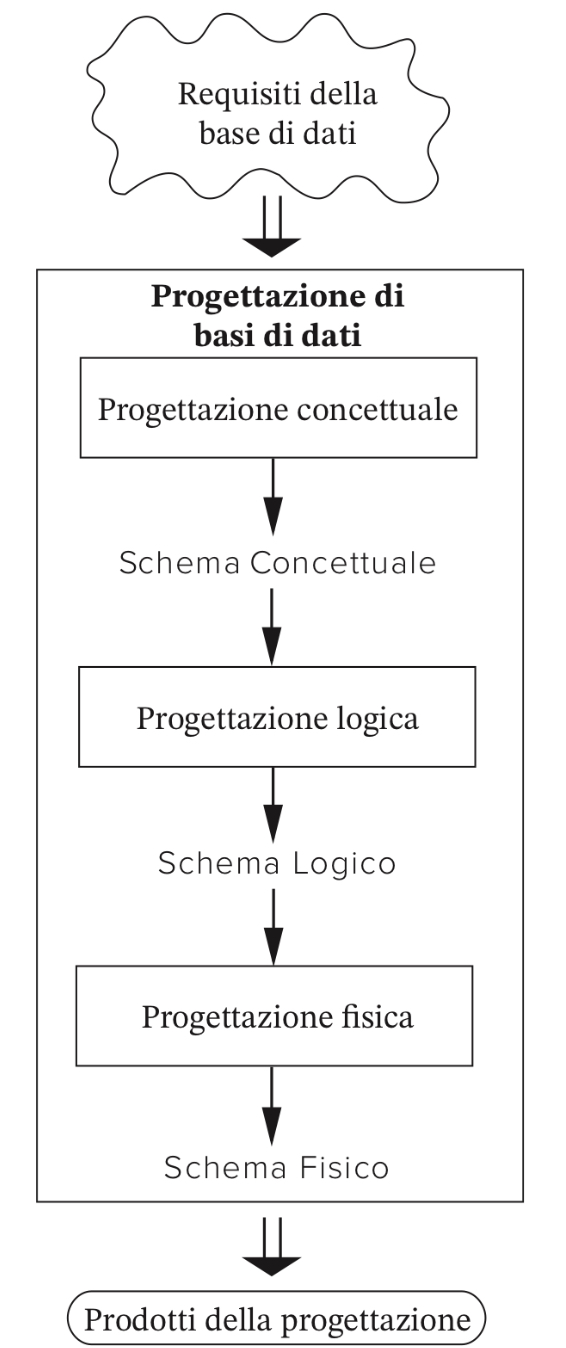
\includegraphics[width=0.2\textwidth, keepaspectratio]{images/progettazioneACascata.jpeg}
      \caption{progettazione a cascata}
    \end{figure}

    \section*{Modello entità-relazione}
    \addcontentsline{toc}{section}{Modello entità-relazione}
    Il \textbf{modello entità-relazione} è un \textit{modello concettuale} di dati e fornisce una serie di strutture (\textit{costrutti}), atte a descrivere la realtà di interesse in una maniera facile da comprendere e che prescinde dai criteri di organizzazione dei dati nei calcolatori.

    Questi costrutti vengono utilizzati per definire \textit{schemi} che descrivono l'organizzazione e la struttura delle \textit{occorenze} dei dati, dei valori assunti dai dati al variare del tempo.

    \subsection*{Entità}
    \addcontentsline{toc}{subsection}{Entità}
    Un'\textbf{entità E} \hl{rappresenta una classe di oggetti} che hanno proprietà comuni ed esistenza "autonoma" ai fini dell'applicazione di interesse (\textit{Città}, \textit{Dipartimento}, \textit{impiegato}, \textit{Acquiesto}, \textit{Vendita} ecc.).

    Un'occorenza di un'entità è un oggetto della classe che l'entità rappresenta (città di Roma, Milano e Palermo sono occorenze dell'entità \textit{Città}).

    Un'occorenza di entità ha un'esistenza indipendente dalle proprietà a esso associate.

    In uno schema, ogni ha un nome che la identifica univocamente e viene rappresentata graficamente mediante un rettangono con il nome dell'intetà all'interno.

    \begin{figure}[H]
      \centering
      \includegraphics[width=0.5\textwidth, keepaspectratio]{images/entità.jpeg}
      \caption{entità}
    \end{figure}

    \subsection*{Relazioni (associazioni)}
    \addcontentsline{toc}{subsection}{Relazioni (associazioni)}
    Una \textbf{relazione R} \hl{rappresneta un legame logico tra due o più entità} (\textit{Residenza} è una relazione che può sussistere tra le entità \textit{Città} e \textit{Impiegato}).

    Un'occorenza di relazione è un'ennupla costituita da occorenze di entità, una per ciascuna delle entità coinvolte.

    In uno schema E-R, ogni relazione ha un nome che identifica univocamente e viene rappresentata graficamente mediante un rombo con il nome delle realzione al'interno e da linee che connettono la relazione con ciascuna delle sue componenti.

    L'insieme delle occorrenze di una relazione del modello E-R è, una relazione matematica tra le occorenze delle enttà coinvolte, ossa, un sottoinsieme del loro prodotto cartesiano.

    Questo significa che tra le occorenze di una relazione del modello E-E non ci possono essere ennuple ripeute.

    \begin{figure}[h]
      \centering

      \begin{subfigure}[b]{0.45\textwidth}
        \centering
        \includegraphics[width=\textwidth, height=3.8cm]{images/relazioniEntità.jpeg}
        \caption{relazioni tra entità}
      \end{subfigure}
      \hfill
      \begin{subfigure}[b]{0.45\textwidth}
        \centering
        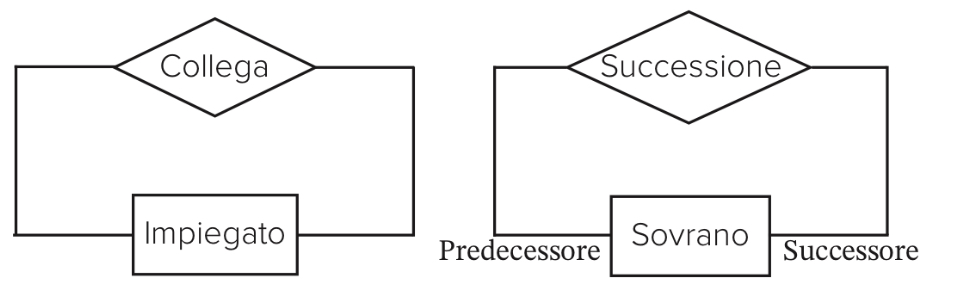
\includegraphics[width=\textwidth, height=3.8cm]{images/relazioniRicorsive.jpeg}
        \caption{relazione ricorsiva}
     \end{subfigure}
    \end{figure}

    E' anche possibile avere \textit{relazioni ricorsive}: relazioni tra un'entità e se stessa.

    E' possibile, infiene, avere \textit{relazioni n-arie} che coinvolgono più di due entità.

    \begin{figure}[H]
      \centering
      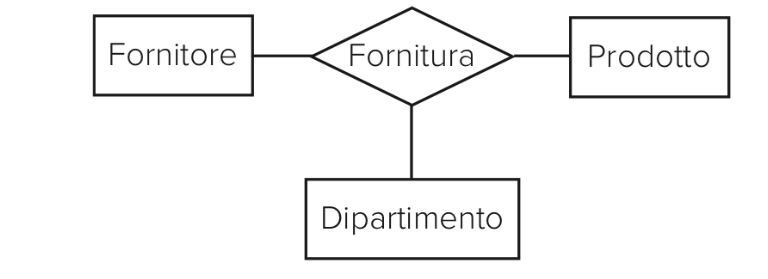
\includegraphics[width=0.5\textwidth, keepaspectratio]{images/relazioneTernaria.jpeg}
      \caption{relazione ternaria}
    \end{figure}

    \subsection*{Attributi}
    \addcontentsline{toc}{subsection}{Attributi}
    Un \textbf{attributo} \hl{descrive le proprietà elementari di un'entità (o relazione)} (\textit{Cognome}, \textit{Stipendio} ed \textit{Età} sono possibili attributi dell'enità \textit{Impiegato}).

    Un attributo associa a ciascuna occorrenza di entità (o di relazione) un valore appartenente a un insieme (\textit{dominio}), che contiene i valori ammissibili per l'attributo.

    I domini non vengono riportati nello shcema, ma sono generalmente nella documentazione associata.

    Può risultare comodo raggruppare attributi della medesima entità (o relazione) che presentano affinità nel loro significto o uso (\textit{attributo composto}), ad esempio \textit{Via}, \textit{Numero civico} e \textit{CAP} possono formare l'attributo composto \textit{Indirrizzo} dell'entità \textit{Persona}.

    \begin{figure}[H]
      \centering
      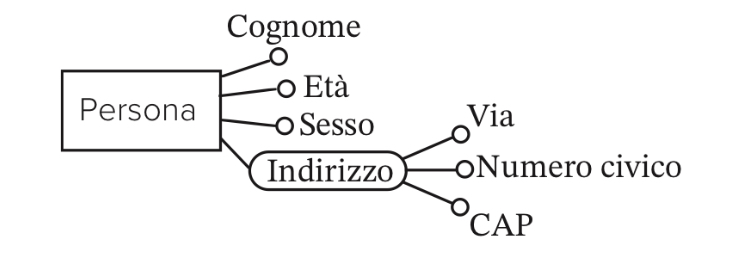
\includegraphics[width=0.5\textwidth, keepaspectratio]{images/attributoComposto.jpeg}
      \caption{attributo composto}
    \end{figure}

    Un esempio completo di \textbf{modello E-R}, può essere il seguente:
    \begin{figure}[H]
      \centering
      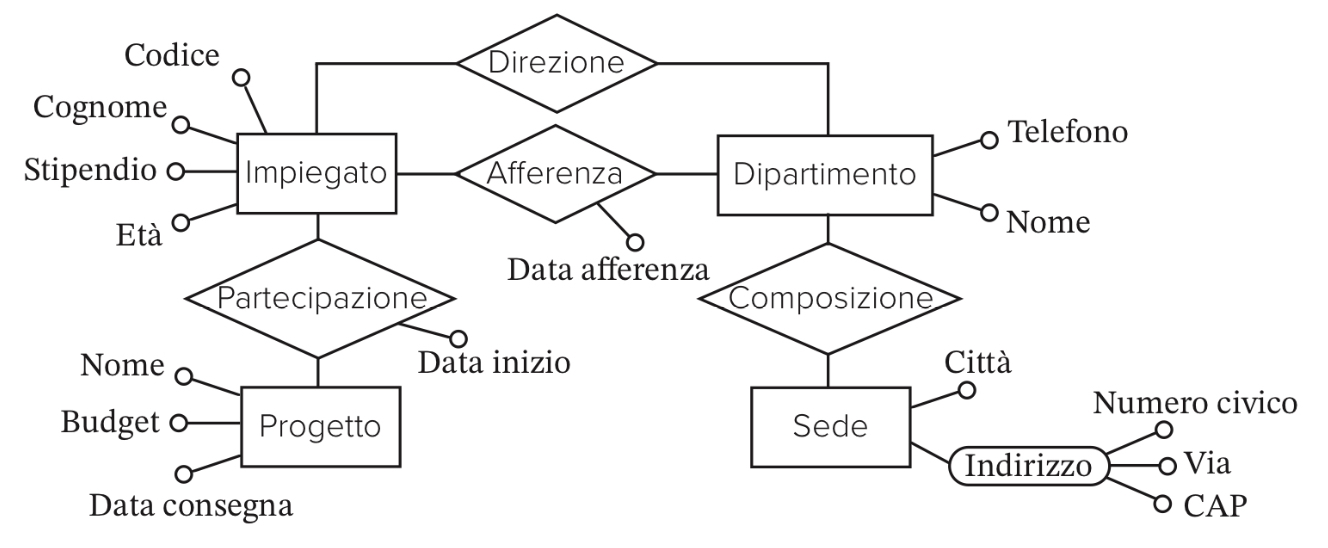
\includegraphics[width=0.5\textwidth, keepaspectratio]{images/modelloE-R.jpeg}
      \caption{modello E-R completo}
    \end{figure}
\end{document}